\begin{frame}
\frametitle{Tête simplifiée / Comparaison FD (différences finies)}
\vfill
\begin{columns}
\column{0.6\textwidth}
\scalebox{0.8}{\begin{minipage}{1.25\textwidth}
\begin{figure}
\begin{tabular}{|l|c|c|}
	\hline
	Critère & GD2-RK2 & FD \\ \hline\hline
	Nombre de mailles & 80 k & 90 M \\	\hline
	Nombre d'inconnues & 13 M & 540 M \\	\hline
	Mémoire & 380 Mo & 9 Go \\	\hline
\end{tabular}
\end{figure}
\begin{itemize}
\item Temps physique simulé : 20 ns ;
\item Corrélation empreinte mémoire - coût de calcul ;
\item Résultats cohérents.
\end{itemize}
\end{minipage}}
\column{0.4\textwidth}
\begin{figure}
	\centering
		Position des points.

			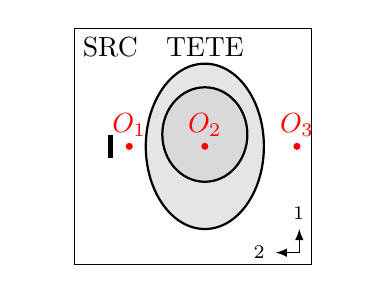
\begin{tikzpicture}[scale=3]
			\fill[white] (-0.2,0) rectangle (1.2,1);
			\draw (0,0) rectangle (1,1);
			\fill (0.14,0.45) rectangle (0.16,0.55);
			\draw[thick,fill=gray!20] (0.55,0.5) ellipse (0.25 and 0.35);
			\draw[thick,fill=gray!30] (0.55,0.55) ellipse (0.18 and 0.2);
			\draw (0.15,1) node[below] {SRC};
			\draw (0.55,1) node[below] {TETE};
			\draw[arrows={-latex}] (0.95,0.05) -- (0.95,0.15) node[above] {$\x_1$};
			\draw[arrows={-latex}] (0.95,0.05) -- (0.85,0.05) node[left] {$\x_2$};
			\fill[red] (0.23,0.5) circle (0.015) node[above,red]{$O_1$};
			\fill[red] (0.55,0.5) circle (0.015) node[above,red]{$O_2$};
			\fill[red] (0.94,0.5) circle (0.015) node[above,red]{$O_3$};
			\end{tikzpicture}
\end{figure}
\end{columns}
\begin{columns}
\column{0.33\textwidth}
\begin{figure}
	\centering
		Au point $O_1$.

			\begin{tikzpicture}[scale=0.5]
			\begin{axis}[
			axis lines=middle,
			xlabel=$t$ (ns), x label style={at={(axis cs:11.5,0)},anchor=south},
			ylabel=$\E$ (V/m), y label style={at={(axis cs:0,6)},anchor=west},
			xmin=0,xmax=13,%ymin=-0.1,ymax=1.1,
			xtick={0,2,...,12},%ytick={0,0.5,1},
			%x post scale=1.8,
			%y post scale=1.2,
			%legend style={at={(axis cs:0.9,0.2)},anchor=south west}
			]
			
			\addplot+[
			%thick,
			mark=none,
			color=red,
			] table
			[y expr=-\thisrowno{1}]
			{../tete_elposd/temsi_ez_O1.plt};
			\addlegendentry{FD}
			
			\addplot+[
			%thick,
			mark=none,
			color=blue,
			densely dashed,
			] table
			{../tete_elposd/teta_ez_O1.plt};
			\addlegendentry{GD}
			
			\end{axis}
			\end{tikzpicture}
\end{figure}
\column{0.33\textwidth}
\begin{figure}
	\centering
		Au point $O_2$.

			\begin{tikzpicture}[scale=0.5]
			\begin{axis}[
			axis lines=middle,
			xlabel=$t$ (ns), x label style={at={(axis cs:11.5,0)},anchor=south},
			ylabel=$\E$ (V/m), y label style={at={(axis cs:0,0.175)},anchor=west},
			xmin=0,xmax=13,%ymin=-0.1,ymax=1.1,
			xtick={0,2,...,12},%ytick={0,0.5,1},
			%x post scale=1.8,
			%y post scale=1.2,
			%legend style={at={(axis cs:0.9,0.2)},anchor=south west}
			]
			
			\addplot+[
			%thick,
			mark=none,
			color=red,
			] table
			[y expr=-\thisrowno{1}]
			{../tete_elposd/temsi_ez_O2.plt};
			\addlegendentry{FD}
			
			\addplot+[
			%thick,
			mark=none,
			color=blue,
			densely dashed,
			] table
			{../tete_elposd/teta_ez_O2.plt};
			\addlegendentry{GD}
			
			\end{axis}
			\end{tikzpicture}
\end{figure}
\column{0.33\textwidth}
\begin{figure}
	\centering
		Au point $O_3$.

			\begin{tikzpicture}[scale=0.5]
			\begin{axis}[
			axis lines=middle,
			xlabel=$t$ (ns), x label style={at={(axis cs:11.5,0)},anchor=south},
			ylabel=$\E$ (mV/m), y label style={at={(axis cs:0,70)},anchor=west},
			xmin=0,xmax=13,%ymin=-0.1,ymax=1.1,
			xtick={0,2,...,12},%ytick={0,0.5,1},
			%x post scale=1.8,
			%y post scale=1.2,
			%legend style={at={(axis cs:0.9,0.2)},anchor=south west}
			]
			
			\addplot+[
			%thick,
			mark=none,
			color=red,
			] table
			[y expr=-\thisrowno{1}*1000]
			{../tete_elposd/temsi_ez_O3.plt};
			\addlegendentry{FD}
			
			\addplot+[
			%thick,
			mark=none,
			color=blue,
			densely dashed,
			] table
			[y expr=\thisrowno{1}*1000]
			{../tete_elposd/teta_ez_O3.plt};
			\addlegendentry{GD}
			
			\end{axis}
			\end{tikzpicture}
\end{figure}
\end{columns}
\vfill
\end{frame}

